\begin{Problem}
	For this programming exercise, you may use Python or any other programming language of your choice. Please write and submit your solution in pdf-format, including excerpts of the core components of your code, the generated plots and figures, as well as comprehensive answers to the following questions:
	
	\begin{enumerate}
		\item[(a)] Generate a list of $N = 10000$ integer random numbers between $0$ and $9$. \hfill (1P)
		
		\item[(b)] Determine the relative frequency of the outcomes and plot them in the form of a histogram (a bar chart with 10 bars). \hfill (2P)
		
		\item[(c)] On average we expect roughly $1000$ outcomes for each digit between $0$ and $9$, corresponding to a relative frequency of $0.1$. What would you roughly expect for the dispersion of the \emph{actual} number of outcomes (that is, the typical size of the random deviation from this average)? \hfill (1P)
		
		\item[(d)] Now let us consider the sum of $K$ uncorrelated random numbers between $0$ and $9$. Obviously, this sum is an integer random number in the range between $0$ and $9K$. Which qualitative shape of the histogram would you expect for $K = 2$? After guessing, modify your code accordingly and generate the histogram by yourself. \hfill (1P)
		
		\item[(e)] What happens to the histogram for large values of $K$? \hfill (1P)
		
	\end{enumerate}
\end{Problem}

\begin{proof}
	The generation of the $N = 10000$ random numbers and the plotting is done in python. The generation was done using the pseudorandom number generator in the random library:
	
	\begin{lstlisting}[language=Python]
		import matplotlib.pyplot as plt
		import numpy as np
		import random
		
		N = 10000
		lst = [random.randint(0,9) for i in range(N)]\end{lstlisting}
	
	The histogram was generated using matplotlib using the following code:
	
	\begin{lstlisting}[language=Python]
		bins = np.arange(0,11) - 0.5
		plt.hist(lst, bins = bins, align = 'mid', rwidth = 0.5)
		plt.gca().set_xticks(range(10))
		plt.gca().set_ylim(ymin=900)\end{lstlisting}

The histogram looks as follows

\begin{center}
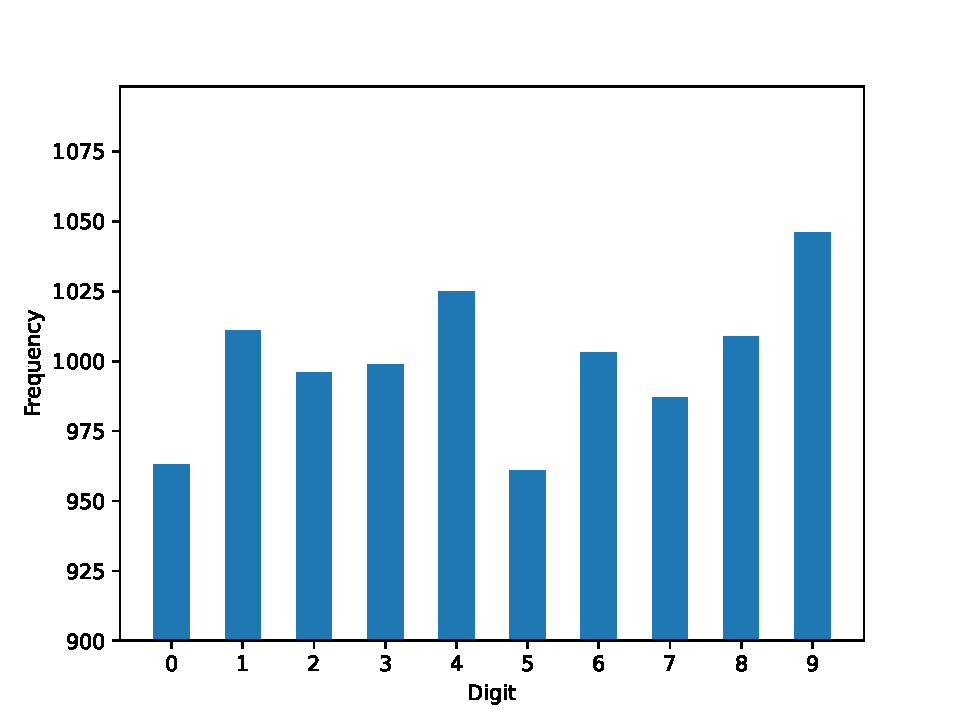
\includegraphics[width=0.5\textwidth]{Sheet 1/histogram.pdf}
\end{center}

The exact counts are 963, 1011,  996,  999, 1025,  961, 1003,  987, 1009, 1046.

In each experiment (generation of a single random digit), all digits can be generated with equal probability $p=1/10$. Thus, if we focus on a single digit $k\in \{0,\dots, 9\}$, the probability that it is generated at each experiment is $p$. The total number of times this digit is generated then follows a binomial distribution with $n(k)\sim B(N, p)$.

It is well known that the standard deviation of a binomial distribution is given by $\sigma=\sqrt{np(1-p)}$. More concretely, using the Moivre-Laplace Theorem, we know that $n(k)$ converges in distribution to a normal distribution $\mathcal{N}(Np, np(1-p))$.

Qualitatively, the distribution should be peaked at the expectation value $9 = 4.5 \cdot 2$, and fall off on both sides, as there are more combinations of possible values near the center as pictured in the diagram below, and the distribution must be symmetric about this expectation value.

\begin{center}
	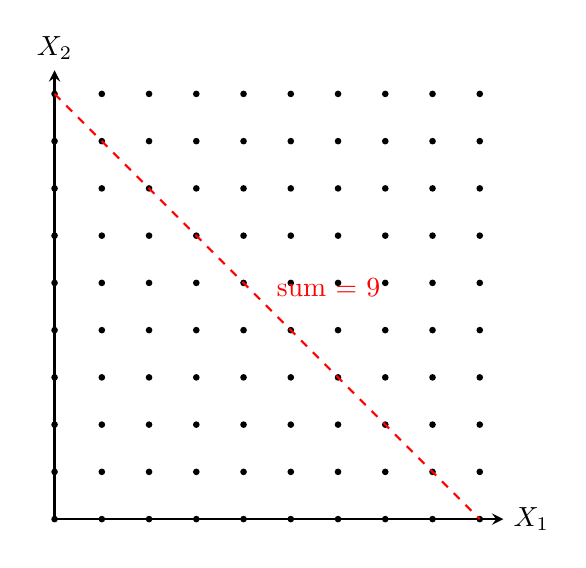
\begin{tikzpicture}[scale=0.6]
		\foreach \x in {0, ..., 9}
		\foreach \y in {0, ..., 9}
		\fill (\x, \y) circle (2pt);
		\draw[thick, -stealth] (0,0) -- (9.5,0) node[anchor=west] {$X_1$};
		\draw[thick, -stealth] (0,0) -- (0,9.5) node[anchor=south] {$X_2$};
		\draw[thick, red, dashed] (0,9) -- (9,0);
		\draw (4.5,4.5) node[anchor=south west, red]{sum = 9};
	\end{tikzpicture}
\end{center}

We generate this analogously

\begin{lstlisting}[language=Python]
	N = 10000
	X1 = np.array([random.randint(0,9) for i in range(N)])
	X2 = np.array([random.randint(0,9) for i in range(N)])
	X3 = X1 + X2
	bins = np.arange(0,20) - 0.5
	plt.hist(X3, bins = bins, align = 'mid', rwidth = 0.5)
	plt.gca().set_xticks(range(19))
	plt.xlabel(r"Sum $X_1+X_2$")
	plt.ylabel("Frequency")\end{lstlisting}

Which yields a histogram as predicted.

\begin{center}
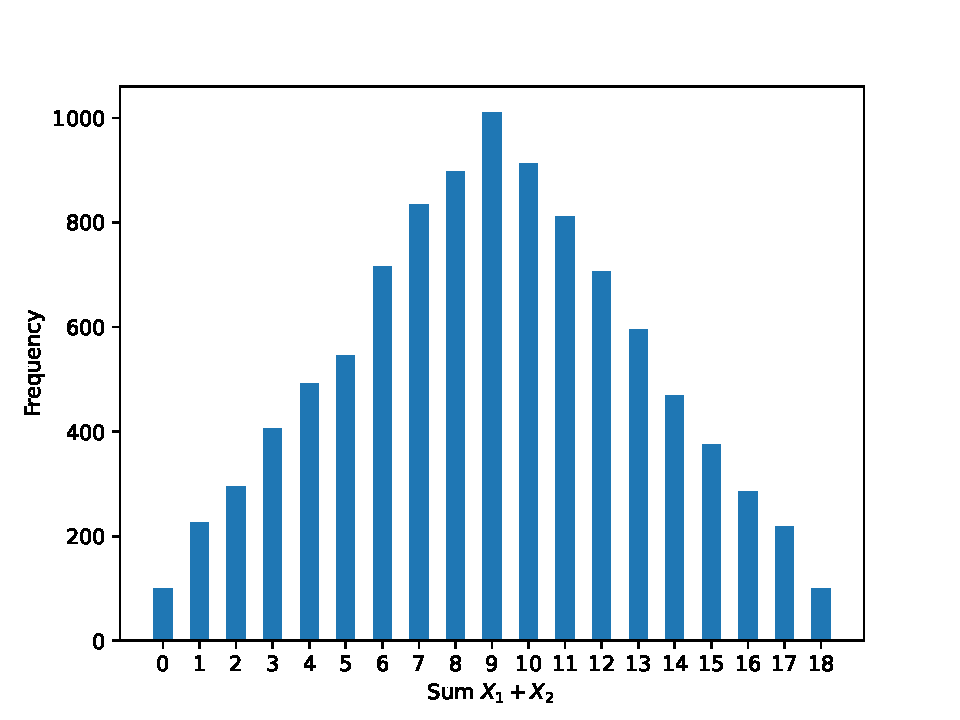
\includegraphics[width=0.5\textwidth]{Sheet 1/histogram_sum.pdf}
\end{center}

For large values of $K$, we have a situation as in the central limit theorem, which states that the sum of iid random variables $S_n = X_1 + \dots + X_n$ converges to a normal distribution in distribution, in the sense that
\[S_n^* := \frac{S_n - n\mu}{\sqrt{n}\sigma}\xrightarrow{d} \mathcal{N}(0,1)\]
where $\mu$ and $\sigma$ are the expected value and standard deviation of the random variables $X$. Thus, we would expect the histogram (after normalisation through division by $K$) to resemble a normal distribution with mean $n\mu$ and standard deviation $\sqrt{n}\sigma$.
\end{proof}